\section{Serial Huffman Algorithm}
\subsection{Priority Queue}
The Huffman algorithm uses a minimum priority queue (MPQ) to build its alphabet efficiently. This specific data structure ensures logarithmic insertion and deletion times with respect to its size.
We implemented the MPQ using a standard C array considered as a minimum heap, by ensuring that the min-heap property holds at every insertion and deletion:
\begin{equation}
    A[i] \le A[l(i)], A[i] \le A[r(i)]
\end{equation}
where \(A[i]\), \(A[l(i)]\), and \(A[r(i)]\) are respectively a node, its left child, and its right child in a min-heap tree.

Also, a parallel approach has been considered to implement to MPQ \cite{BRODAL19984}, but it has been discarded since very complex and without any practical gain since we are dealing with MPQ of at most 256 elements.

\subsection{Encoding}
The Huffman encoding procedure makes use of a MPQ to build its alphabet efficiently. The idea is to build a tree similar to \cref{fig:tree} that defines all the variable-length prefix sequences of bits: these sequences are represented by the path from the tree root to a leaf. Using a greedy approach, the Huffman encoding ensures that the less frequent a byte is in a file, the more probable is to have a longer Huffman representation, which means that his path from the root to its specific leaf is longer.

Once having computed the frequencies for each one of the 256 different bytes in a file, the Huffman algorithm populates a min priority queue with Huffman tree nodes storing the byte value and its frequency. Successively, it removes the least two frequent bytes from the queue, creates a new node with children the two extracted nodes, assigns to it a dummy character and the sum of the frequencies of its two children, and inserts it into the min priority queue. After \(n-1\) iterations, the last node is the root of the Huffman tree \cite{bertossi2010algoritmi}. \Cref{alg:buildtree} explains in the detail this procedure.
\begin{algorithm}
    \caption{Build the Huffman tree}\label{alg:buildtree}

    \SetKwData{Q}{Q}\SetKwData{z1}{z1}\SetKwData{z2}{z2}\SetKwData{z}{z}
    \SetKwFunction{insert}{insert}\SetKwFunction{deleteMin}{deleteMin}
    \SetKwInOut{Input}{input}\SetKwInOut{Output}{output}
    \SetKwFor{}{}{}{}

    // Populate the min priority queue with characters and their frequencies\;
    \For{\(i=1\) \KwTo \(n-1\)}{
        Q.insert(f[i], Tree(f[i], c[i]))\;
    }
    // Repeat until the queue has only a single element left\;
    \For{\(i=1\) \KwTo \(n-1\)}{
        // Get the two least frequent nodes\;
        z1, z2 = Q.deleteMin(), Q.deleteMin()\;

        // Create and insert inner tree node into the queue\;
        z = Tree(z1.f + z2.f, null)\;
        z.left, z.right = z1, z2\;
        Q.insert(z.f, z)\;
    }

    // The last element in the queue is the root of the Huffman tree\;
    \Return{Q.deleteMin()}\;
\end{algorithm}

Once built the Huffman tree, it is possible to generate the Huffman alphabet visiting the tree using a DFS algorithm, assigning 0 to each left-child traverse and 1 for the right one as presented in \cref{alg:encode}. Finally, it is possible to compress the file by creating a stream of bits corresponding to its content using the Huffman alphabet.

\begin{algorithm}
    \caption{Encode(node)}\label{alg:encode}
    \While{not eof()}{
        bit = read()\;
        \eIf{bit == 0}{
            Encode(node.left)\;
        }{
            Encode(node.right)\;
        }
        \If{node is leaf}{
            \Return{node.value}\;
        }
    }
\end{algorithm}

\begin{center}
    \begin{figure}
        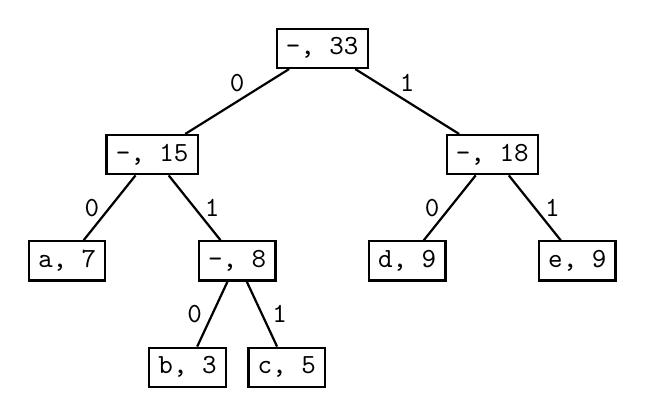
\begin{tikzpicture}
            [
                level distance=1.5cm,
                level 1/.style={sibling distance=4.8cm},
                level 2/.style={sibling distance=2.4cm},
                level 3/.style={sibling distance=1.4cm},
                thick,
                font=\ttfamily\bfseries, scale=0.9
            ]
            \tikzset{
                treenode/.style = {rectangle, draw=black, align=center,minimum width=0.75cm},
                edgestyleL/.style = {midway,left,draw=none},
                edgestyleR/.style = {midway,right,draw=none}
            }
            \node [treenode] (T) {-, 33}
            child { node[treenode] (L) {-, 15}
                    child { node[treenode] (LL) {a, 7} edge from parent node[edgestyleL] {0} }
                    child { node[treenode] (LR) {-, 8}
                            child { node[treenode] (LRL) {b, 3} edge from parent node[edgestyleL] {0} }
                            child { node[treenode] (LRR) {c, 5} edge from parent node[edgestyleR] {1} }
                            edge from parent node[edgestyleR] {1}
                        }
                    edge from parent node[edgestyleL,above] {0}
                }
            child { node[treenode] (R) {-, 18}
                    child { node[treenode] {d, 9} edge from parent node[edgestyleL] {0}}
                    child { node[treenode] {e, 9} edge from parent node[edgestyleR] {1}}
                    edge from parent node[edgestyleR,above] {1}
                }
            ;
        \end{tikzpicture}
        \caption{An example of Huffman tree.}
        \label{fig:tree}
    \end{figure}

\end{center}

\subsection{Decoding}
Once having the encoded file and the Huffman tree, it is straightforward to decompress the file to its original shape. The prefix alphabet ensures to have that it is possible to visit the tree using a DFS approach and get a unique decoded version of the file using an approach similar to \cref{alg:encode}.

\subsection{Implementation}
To be able to implement the Huffman encoding and decoding algorithm, several things have been taken into account.
\begin{itemize}
    \item The byte frequencies computed during the encoding process are saved in the compressed file. In this way, the decoding procedure can easily rebuild the Huffman tree.
    \item Both the encoding and decoding procedures make use of buffers to improve I/O performance: the streams of bytes are first written inside the buffer and then saved on the disk.
    \item The encoding procedure works with chunks of \(4096\) bytes. This ensures that the tool can handle even large files when dealing with bit buffers. The decoding procedure deals with chunks of maximum size of \(4096*32\) bytes, since the maximum length of a Huffman tree traverse from root to leaf is of 256 bits, which is 32 times a byte. As explained later, dealing with chunks makes handy the parallel implementation of the encoding and decoding algorithms.
    \item In the encoded file, the chunk offsets are saved at the end of the file: this ensures that the compressed stream of prefixed sequences of bits is still meaningful.
\end{itemize}
